\section{Microwind}

Microwind to zintegrowane oprogramowanie należące do rodziny EDA (ang. \textit{Electronic Design Automation}),
służące do automatyzacji procesu projektowania układów scalonych lub płytek drukowanych,
umożliwiające projektowanie, symulacje, weryfikacje oraz testowanie układów elektronicznych~\cite{eda}.
Program ten został opracowany przez dra Sicarda do celów edukacyjnych, składa się z kilku modułów,
odpowiadających za różne etapy projektowania układów scalonych~\cite{Microwind}.
Instalacja w przypadku Microwinda jest prosta, wymaga jedynie pobrania pliku instalacyjnego z oficjalnej strony,
a następnie zainstalowania go na komputerze z systemem Windows~\cite{Microwind},
są to natomiast wersje lite (wersja z ograniczoną funkcjonalnością), pełna wersja wymaga licencji.
Dostępna jest także archiwalna pełna wersja programu, która jest dostępna za darmo~\cite{old_microwind}.
Strona zawiera również dokumentację oraz przykłady projektów,
które można wykorzystać w celach edukacyjnych~\cite{Microwind}.\\
\indent Jednym z modułów programu Microwind jest edytor schematów \textbf{Nano Lambda},
pojawiający się domyślnie po uruchomieniu programu.
Posiada dość nieskomplikowany interfejs graficzny z paskiem menu i narzędzi
oraz pływającym oknem palety warstw, przedstawiony na rys.~\ref{fig:microwind_okno}.

\begin{figure}[h]
    \centering
    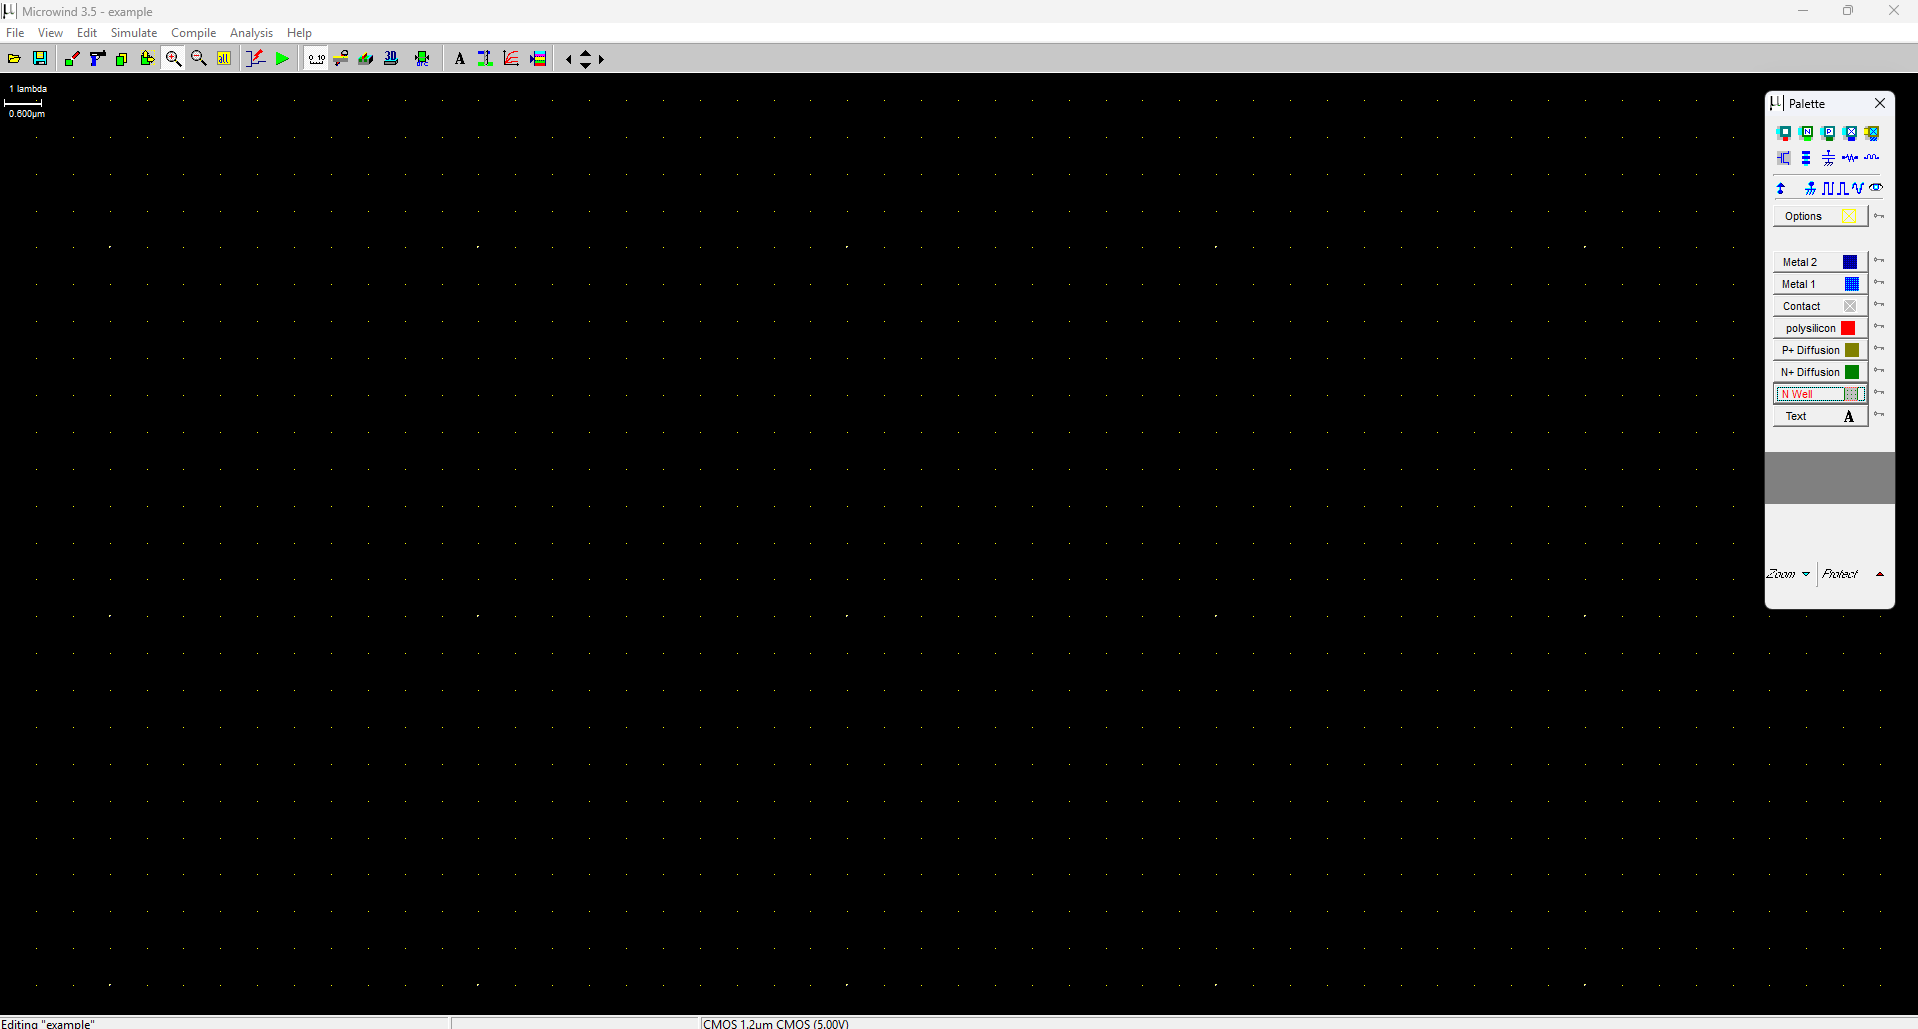
\includegraphics[width=.9\textwidth]{chapters/chapter2/img/microwind_okno}
    \caption[Widok głównego okna programu Microwind.]{Widok głównego okna programu Microwind, źródło:~\cite{Microwind}.}
    \label{fig:microwind_okno}
\end{figure}

\indent Rysowanie odbywa się podobnie jak w przypadku klasycznych edytorów graficznych,
poprzez wybór warstwy z palety,
a następnie przeciągając kursorem po obszarze roboczym przy wciśniętym lewym lub środkowym przycisku myszy,
rysując przy tym prostokątną komórkę.
Nieznaczną wadą rysowania w Microwindzie jest brak przyciągania do siatki,
przez co jest mało precyzyjne.
Przemieszczanie się na obszarze roboczym wymaga używania klawiszy kierunkowych lub przycisków na pasku narzędzi,
co obecnie jest już rozwiązaniem nieergonomicznym.
Program Microwind, poza typowymi narzędziami edycji, charakteryzuje się wieloma zautomatyzowanymi narzędziami,
pozwalającymi generowanie elementów schematów,
na przykład na podstawie funkcji logicznych lub kodu Verilog~\cite{microwind_operation_commands}.\\
\indent Ze względu na brak otwartego kodu źródłowego trudno określić dokładnie zastosowane mechanizmy edytora,
natomiast na podstawie obserwacji można stwierdzić,
że każda edycja schematu wywołuje ponowne rysowanie całego obszaru roboczego,
co jest szczególnie zauważalne podczas usuwania komórek.
Ta sama operacja również wskazuje na strukturę danych, która zakotwiczeniu komórek w kolumnach,
ponieważ po usunięciu obszaru wewnątrz większej komórki, cała kolumna zostaje usunięta.\\
% TODO: poniższe poprawić
\indent Szata graficzna samego edytora charakteryzuje się wysokim kontrastem,
gdzie warstwy są jednolitymi kolorami, częściowo przezroczystymi,
co jest zauważalne, gdy warstwy te się nakładają, przykład przedstawiono na rys.~\ref{fig:microwind_tran}.

\begin{figure}[h]
    \centering
    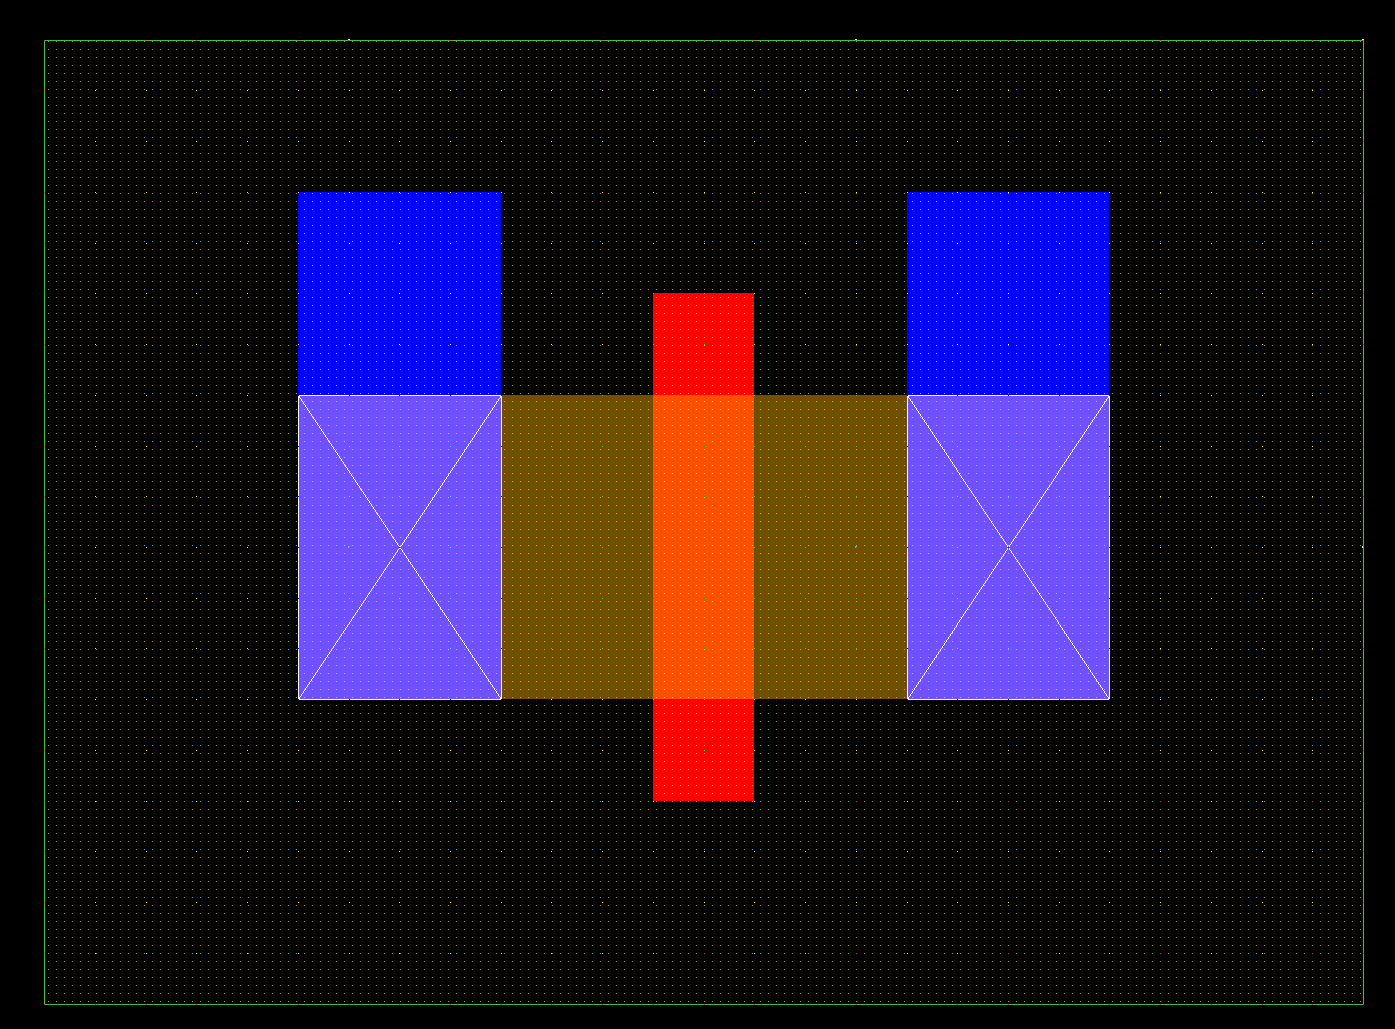
\includegraphics[width=.9\textwidth]{chapters/chapter2/img/microwind_tran}
    \caption[Przykład tranzystora narysowanego w programie Microwind.]
    {
        Przykład tranzystora narysowanego w programie Microwind,
        warstwy \textit{Metal 1}, \textit{P+ Diffusion} oraz \textit{Polysilicon} są jednoilitymi kolorami,
        z wyjątkiem warstwy \textit{N Well} którą reprezentuje kropkowany wzór,
        , źródło: opracowanie własne.
    }
    \label{fig:microwind_tran}
\end{figure}
